
%(BEGIN_QUESTION)
% Copyright 2011, Tony R. Kuphaldt, released under the Creative Commons Attribution License (v 1.0)
% This means you may do almost anything with this work of mine, so long as you give me proper credit

Explain why no one in their right mind would ever, {\it ever}, install a three-valve manifold on a DP transmitter with remote seals:

$$\includegraphics[width=15.5cm]{i03460x01.eps}$$

\underbar{file i03460}
%(END_QUESTION)





%(BEGIN_ANSWER)

If the equalizing valve is ever opened, it could shuttle fill fluid from one remote seal to the other, imbalancing the system.  This would make the transmitter read less differential pressure than there actually was applied between the remote seals.  The problem would be difficult to correct without dismantling the system entirely and re-packing the seals and capillary tubes with fill fluid.

%(END_ANSWER)





%(BEGIN_NOTES)


%INDEX% Measurement, pressure: 3-valve manifold operation

%(END_NOTES)

